
\documentclass[aspectratio=169,11pt]{beamer}

% -------------------------------------------------
% Packages
% -------------------------------------------------
\usepackage{amsmath,amssymb}
\usepackage{booktabs,array,tabularx,multirow}
\usepackage{graphicx}
\usepackage{tikz}
\usepackage{pgfplots}
\usepackage{siunitx}
\usepackage{ragged2e}
\usetikzlibrary{arrows.meta, positioning, shapes.geometric, fit, calc, shadows.blur}
\pgfplotsset{compat=1.18}

\sisetup{
  detect-all,
  per-mode=symbol,
  range-phrase=--,
  range-units=single
}

% -------------------------------------------------
% Theme and colors
% -------------------------------------------------
\usetheme{Boadilla}
\usecolortheme{dolphin}
\setbeamertemplate{navigation symbols}{}
\setbeamertemplate{footline}[frame number]

\definecolor{navydeep}{RGB}{10,72,110}
\definecolor{navymain}{RGB}{28,114,147}
\definecolor{tealaccent}{RGB}{34,139,136}
\definecolor{iceblue}{RGB}{236,244,251}
\definecolor{lightblue}{RGB}{206,224,248}

\setbeamercolor{structure}{fg=navymain}
\setbeamercolor{frametitle}{bg=navymain,fg=white}
\setbeamercolor{title}{fg=white}
\setbeamercolor{subtitle}{fg=white}
\setbeamercolor{block title}{bg=navymain,fg=white}
\setbeamercolor{block body}{bg=iceblue,fg=black}
\setbeamercolor{block title alerted}{bg=navydeep,fg=white}
\setbeamercolor{block body alerted}{bg=navydeep!7,fg=black}
\setbeamercolor{block title example}{bg=tealaccent,fg=white}
\setbeamercolor{block body example}{bg=tealaccent!8,fg=black}

\setbeamertemplate{itemize item}{\color{navymain}$\blacktriangleright$}
\setbeamertemplate{itemize subitem}{\color{navydeep}$\small\blacktriangleright$}
\setlength{\parskip}{0.20em}

% -------------------------------------------------
% Helpers
% -------------------------------------------------
\newcommand{\ok}{\textcolor{green!50!black}{\checkmark}}
\newcommand{\cadplaceholder}[1]{%
\begin{center}
\fbox{%
\parbox[c][0.16\textheight][c]{0.92\linewidth}{\centering\small\textcolor{navymain}{\textbf{#1}}}%
}
\end{center}
}

% -------------------------------------------------
% Metadata
% -------------------------------------------------
\title[\textbf{Fixed-Wing UAV for Emergency Medical Delivery}]{\textbf{Fixed-Wing UAV for Emergency Medical Delivery}}
\subtitle{AS5213: Conceptual Design of UAVs}
\author{DS Vivek \and Divyam Pandey \and G. Vishwas \and Manav Agarwal \and Monisha V \and Abhijeet Mangela}
\institute{Group 11: Skunk Works\\Department of Aerospace Engineering\\IIT Madras}
\date{April 2026}

\graphicspath{{./}}

% -------------------------------------------------
\begin{document}

% -------------------------------------------------
\begin{frame}[plain]
  \setbeamercolor{background canvas}{bg=navydeep}
  \begin{tikzpicture}[remember picture,overlay]
    \fill[navydeep] (current page.south west) rectangle (current page.north east);
    \fill[white,opacity=0.08] ([xshift=-1cm,yshift=1.4cm]current page.south east) circle (4.5cm);
    \fill[white,opacity=0.06] ([xshift=2cm,yshift=-1.0cm]current page.north west) circle (5.5cm);
  \end{tikzpicture}

  \vspace*{0.35cm}
  \begin{center}
    {\color{white}\fontsize{18}{21}\selectfont\bfseries Fixed-Wing UAV for Emergency Medical Delivery\par}
    \vspace{0.15cm}
    {\large\color{white}AS5213: Conceptual Design of UAVs\par}
    \vspace{0.25cm}
    {\color{white}\small Group 11: Skunk Works \\ Department of Aerospace Engineering \\ IIT Madras\par}
    \vspace{0.25cm}
    \begin{beamercolorbox}[rounded=true,shadow=true,wd=0.78\textwidth,center,sep=0.55em]{block body}
      \textcolor{navymain}{\textbf{Concept snapshot:}} time-critical medical delivery, STOL operation, droppable payload, and stable cruise between remote sites.
    \end{beamercolorbox}
    \vspace{0.25cm}
    \fbox{\parbox[c][0.13\textheight][c]{0.70\textwidth}{\centering\color{white}\textbf{Placeholder: Isometric CAD render}}}
  \end{center}
\end{frame}

% -------------------------------------------------
\begin{frame}[t]{Presentation Roadmap}
\small
\begin{columns}[T,onlytextwidth]
  \column{0.48\textwidth}
  \begin{block}{Mission and concept}
  \begin{itemize}
    \item Mission profile and requirements
    \item Design methodology
    \item Aircraft configuration
  \end{itemize}
  \end{block}

  \begin{block}{Technical data}
  \begin{itemize}
    \item Powerplant and energy budget
    \item Aerodynamic parameters
    \item Mass properties and inertia
  \end{itemize}
  \end{block}

  \column{0.48\textwidth}
  \begin{block}{Verification}
  \begin{itemize}
    \item Performance envelope
    \item Stability and eigenvalues
    \item Requirements compliance
  \end{itemize}
  \end{block}

  \begin{alertblock}{Goal}
  Show that the UAV meets mission range, payload, STOL, and stability targets with a practical conceptual design.
  \end{alertblock}
\end{columns}
\end{frame}

% -------------------------------------------------
\begin{frame}[t]{Mission Requirements}
\begin{columns}[T,onlytextwidth]
  \column{0.54\textwidth}
  \begin{block}{Mission objective}
  \small
  A fixed-wing UAV to deliver antivenom and blood products to remote locations with a droppable payload and return capability.
  \end{block}

  \begin{block}{Top-level requirements}
  \small
  \begin{itemize}
    \item Wingspan limited to \SI{2.00}{\meter}
    \item Payload mass around \SI{1}{\kilogram}
    \item Operational radius \SIrange{40}{50}{\kilo\meter}
    \item Total range \SIrange{80}{100}{\kilo\meter}
    \item Cruise speed \SIrange{18}{25}{\meter\per\second}
    \item Takeoff distance below \SI{150}{\meter}
  \end{itemize}
  \end{block}

  \column{0.42\textwidth}
  \begin{exampleblock}{Mission phases}
  \small
  \begin{enumerate}
    \item Takeoff and climb
    \item Outbound cruise
    \item Payload drop
    \item Return cruise
    \item Descent and landing
  \end{enumerate}
  \end{exampleblock}

  \begin{beamercolorbox}[rounded=true,wd=\linewidth,sep=0.55em,center]{block body}
    \textcolor{navymain}{\textbf{Design driver:}} range and payload have to remain compatible with STOL operation.
  \end{beamercolorbox}
\end{columns}
\end{frame}

% -------------------------------------------------
\begin{frame}[t]{Mission Profile}
\begin{figure}
  \centering
  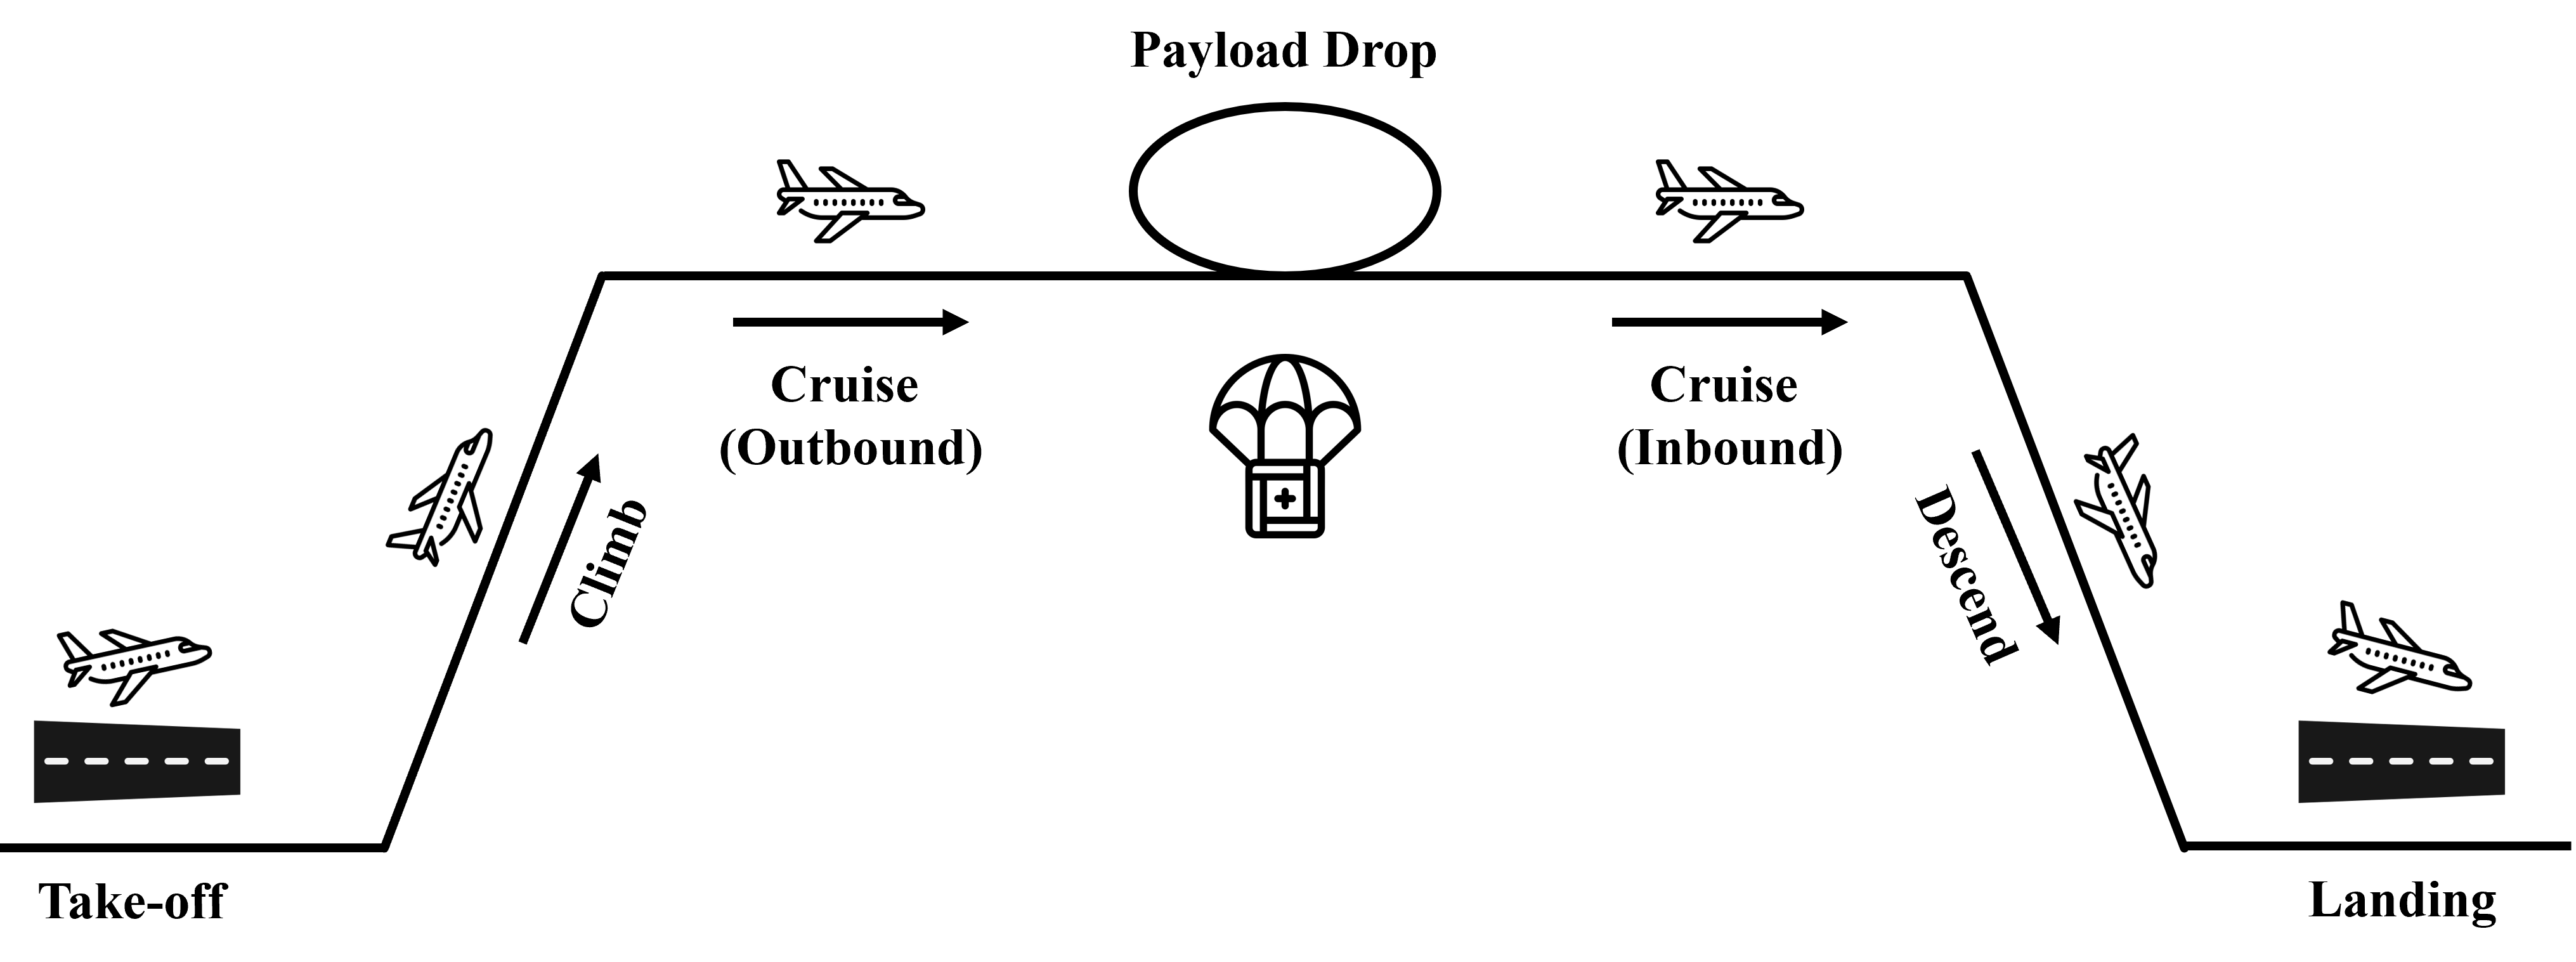
\includegraphics[width=\linewidth,height=0.74\textheight,keepaspectratio]{Mission Profile_new.png}
\end{figure}
\vspace{-0.8em}
{\footnotesize\centering Mission timeline used to size propulsion, energy storage, and payload-drop events.\par}
\end{frame}

% -------------------------------------------------
\begin{frame}[t]{Design Methodology}
\centering
\resizebox{0.82\textwidth}{!}{%
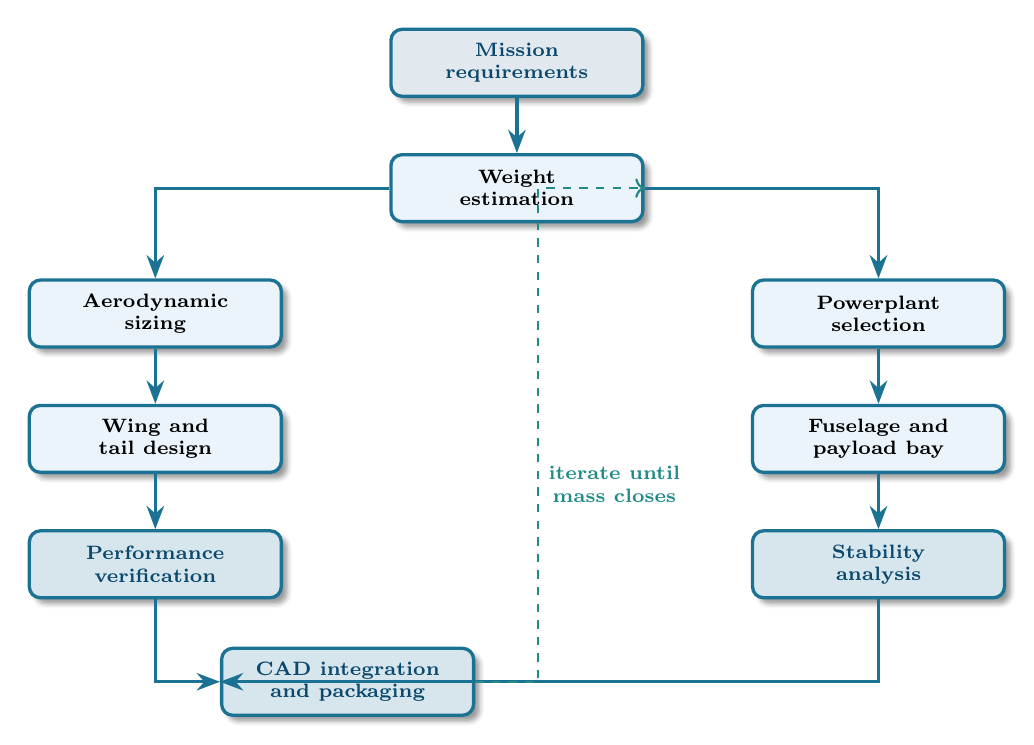
\begin{tikzpicture}[
    node distance=7mm and 12mm,
    box/.style={
      rectangle,
      rounded corners=4pt,
      draw=navymain,
      very thick,
      align=center,
      minimum width=3.20cm,
      minimum height=0.85cm,
      fill=white,
      font=\bfseries\scriptsize,
      blur shadow
    },
    start/.style={box, fill=navydeep!12, text=navydeep},
    process/.style={box, fill=iceblue, text=black},
    result/.style={box, fill=navymain!18, text=navydeep},
    arrow/.style={->, very thick, >=Stealth, color=navymain}
]
\node[start] (req) {Mission\\requirements};
\node[process, below=of req] (weight) {Weight\\estimation};
\node[process, below left=of weight, xshift=-0.15cm] (aero) {Aerodynamic\\sizing};
\node[process, below right=of weight, xshift=0.15cm] (power) {Powerplant\\selection};
\node[process, below=of aero] (wing) {Wing and\\tail design};
\node[process, below=of power] (fuse) {Fuselage and\\payload bay};
\node[result, below=of wing] (perf) {Performance\\verification};
\node[result, below=of fuse] (stab) {Stability\\analysis};
\node[result, below right=0.6cm and -0.8cm of perf] (cad) {CAD integration\\and packaging};

\draw[arrow] (req) -- (weight);
\draw[arrow] (weight) -| (aero);
\draw[arrow] (weight) -| (power);
\draw[arrow] (aero) -- (wing);
\draw[arrow] (power) -- (fuse);
\draw[arrow] (wing) -- (perf);
\draw[arrow] (fuse) -- (stab);
\draw[arrow] (perf) |- (cad.west);
\draw[arrow] (stab) |- (cad.west);
\draw[->, thick, dashed, color=tealaccent]
(cad.east) -- ++(0.8,0) |- node[pos=0.20, right, align=center, font=\scriptsize\bfseries, text=tealaccent]
{iterate until\\mass closes} (weight.east);
\end{tikzpicture}%
}
\end{frame}

% -------------------------------------------------
\begin{frame}[t]{Technical Data I: Powerplant}
\begin{columns}[T,onlytextwidth]
  \column{0.56\textwidth}
  \begin{block}{Propulsion and energy system}
  \small
  \renewcommand{\arraystretch}{1.12}
  \begin{tabular}{@{}>{\bfseries}p{0.37\linewidth}p{0.56\linewidth}@{}}
    \toprule
    Motor & T-Motor AM480 900KV \\
    Configuration & Dual tractor motors \\
    Maximum power & \SI{450}{\watt} at 80\% throttle \\
    Supply voltage & \SI{11.1}{\volt} (3S LiPo) \\
    Peak current & \SI{26}{\ampere} \\
    ESC & Hobbywing Skywalker 50A V2 \\
    Propeller & APC 12$\times$6E \\
    \bottomrule
  \end{tabular}
  \end{block}

  \begin{exampleblock}{Power budget}
  \small
  Climb power: \SI{361.46}{\watt}\qquad Avionics: \SI{6.61}{\watt}\\
  Battery efficiency: 85\%\qquad Motor efficiency: 82\%
  \end{exampleblock}

  \column{0.40\textwidth}
  \begin{block}{Component imagery}
  \centering
  \cadplaceholder{Motor / propeller / battery images were not provided}
  \end{block}

  \begin{alertblock}{Installation note}
  \small
  Dual-tractor wing-mounted propulsion with the battery placed to help CG control.
  \end{alertblock}
\end{columns}
\end{frame}

% -------------------------------------------------
\begin{frame}[t]{Technical Data II: Aerodynamics}
\begin{columns}[T,onlytextwidth]
  \column{0.43\textwidth}
  \begin{block}{Wing and drag data}
  \small
  \renewcommand{\arraystretch}{1.10}
  \begin{tabular}{@{}>{\bfseries}p{0.50\linewidth}p{0.42\linewidth}@{}}
    \toprule
    Airfoil & Selig S7055 \\
    Planform & Rectangular, high-wing \\
    Aspect ratio & 7.53 \\
    Wing area & \SI{0.5307}{\meter\squared} \\
    Wingspan & \SI{2.00}{\meter} \\
    Mean chord & \SI{0.2653}{\meter} \\
    Zero-lift drag & $C_{D_0}=0.02873$ \\
    Oswald efficiency & $e=0.85$ \\
    Max L/D & 12.55 \\
    \bottomrule
  \end{tabular}
  \end{block}

  \column{0.55\textwidth}
  \begin{columns}[T,onlytextwidth]
    \column{0.5\textwidth}
    \begin{figure}
      \centering
      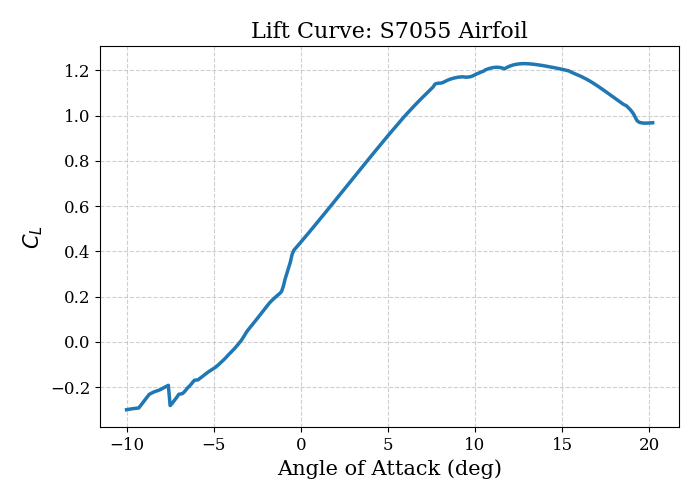
\includegraphics[width=\linewidth,height=0.25\textheight,keepaspectratio]{cl_alp.png}
      \par\vspace{0.15em}
      {\footnotesize Lift curve}
    \end{figure}
    \column{0.5\textwidth}
    \begin{figure}
      \centering
      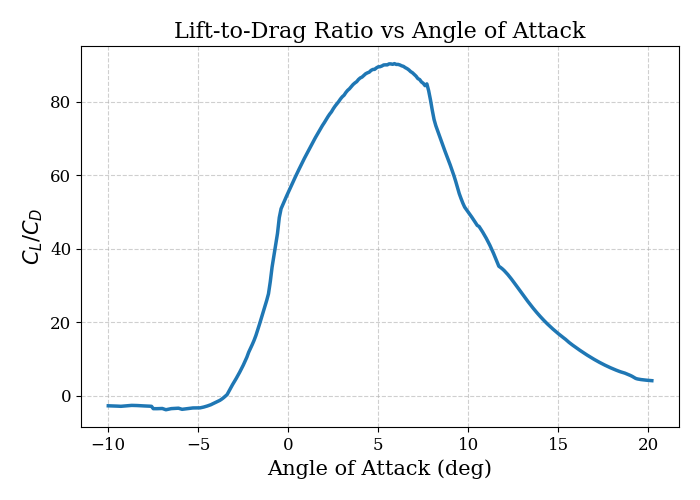
\includegraphics[width=\linewidth,height=0.25\textheight,keepaspectratio]{CL_Cd_alpha.png}
      \par\vspace{0.15em}
      {\footnotesize $C_L/C_D$ vs. angle of attack}
    \end{figure}
  \end{columns}

  \begin{exampleblock}{Key result}
  \small
  \(C_{L_\alpha} = \SI{5.73}{\per\radian}\), cruise \(C_L \approx 0.65\)--0.75, and estimated stall speed \SI{12.4}{\meter\per\second}.
  \end{exampleblock}
\end{columns}
\end{frame}

% -------------------------------------------------
\begin{frame}[t]{Technical Data III: Mass Properties}
\begin{columns}[T,onlytextwidth]
  \column{0.50\textwidth}
  \begin{block}{Mass breakdown}
  \small
  \renewcommand{\arraystretch}{1.08}
  \begin{tabular}{@{}>{\bfseries}p{0.50\linewidth}p{0.34\linewidth}@{}}
    \toprule
    MTOW & \SI{6.59}{\kilo\gram} \\
    Empty weight & \SI{3.29}{\kilo\gram} \\
    Battery & \SI{0.987}{\kilo\gram} \\
    Payload & \SI{1.20}{\kilo\gram} \\
    Avionics & \SI{0.90}{\kilo\gram} \\
    Empty fraction & 0.50 \\
    Static margin & \(\approx 14\%\) MAC \\
    \bottomrule
  \end{tabular}
  \end{block}

  \begin{block}{Geometry}
  \small
  \begin{tabular}{@{}>{\bfseries}p{0.50\linewidth}p{0.34\linewidth}@{}}
    \toprule
    Fuselage length & \SI{1.10}{\meter} \\
    Fuselage diameter & \SI{0.15}{\meter} \\
    Tail boom length & \SI{0.70}{\meter} \\
    CG location & \SI{264}{\milli\meter} from nose \\
    Neutral point & \SI{296}{\milli\meter} \\
    \bottomrule
  \end{tabular}
  \end{block}

  \column{0.48\textwidth}
  \begin{block}{Empennage and controls}
  \small
  \begin{tabular}{@{}>{\bfseries}p{0.56\linewidth}p{0.30\linewidth}@{}}
    \toprule
    Horizontal tail area & \SI{0.133}{\meter\squared} \\
    Horizontal tail span & \SI{0.773}{\meter} \\
    Tail arm & \SI{0.70}{\meter} \\
    Tail airfoil & NACA 0012 \\
    Tail setting angle & \(-0.31^\circ\) \\
    Vertical tail area & \SI{0.080}{\meter\squared} \\
    \bottomrule
  \end{tabular}
  \end{block}

  \begin{alertblock}{Design note}
  The payload bay is placed near the CG and supports droppable payload release without destabilizing the aircraft.
  \end{alertblock}
\end{columns}
\end{frame}

% -------------------------------------------------
\begin{frame}[t]{Performance I: Power Required}
\begin{columns}[T,onlytextwidth]
  \column{0.36\textwidth}
  \begin{block}{Performance summary}
  \small
  \begin{itemize}
    \item Cruise speed: \SIrange{18}{22}{\meter\per\second}
    \item Maximum range: \SI{83.15}{\kilo\meter}
    \item Endurance: 2 h 5 min
    \item Service ceiling: \SI{2000}{\meter}
    \item Maximum speed: \SI{28}{\meter\per\second}
  \end{itemize}
  \end{block}

  \begin{exampleblock}{Power margin}
  \small
  The required power remains below available power across the practical cruise band.
  \end{exampleblock}

  \column{0.62\textwidth}
  \begin{figure}
    \centering
    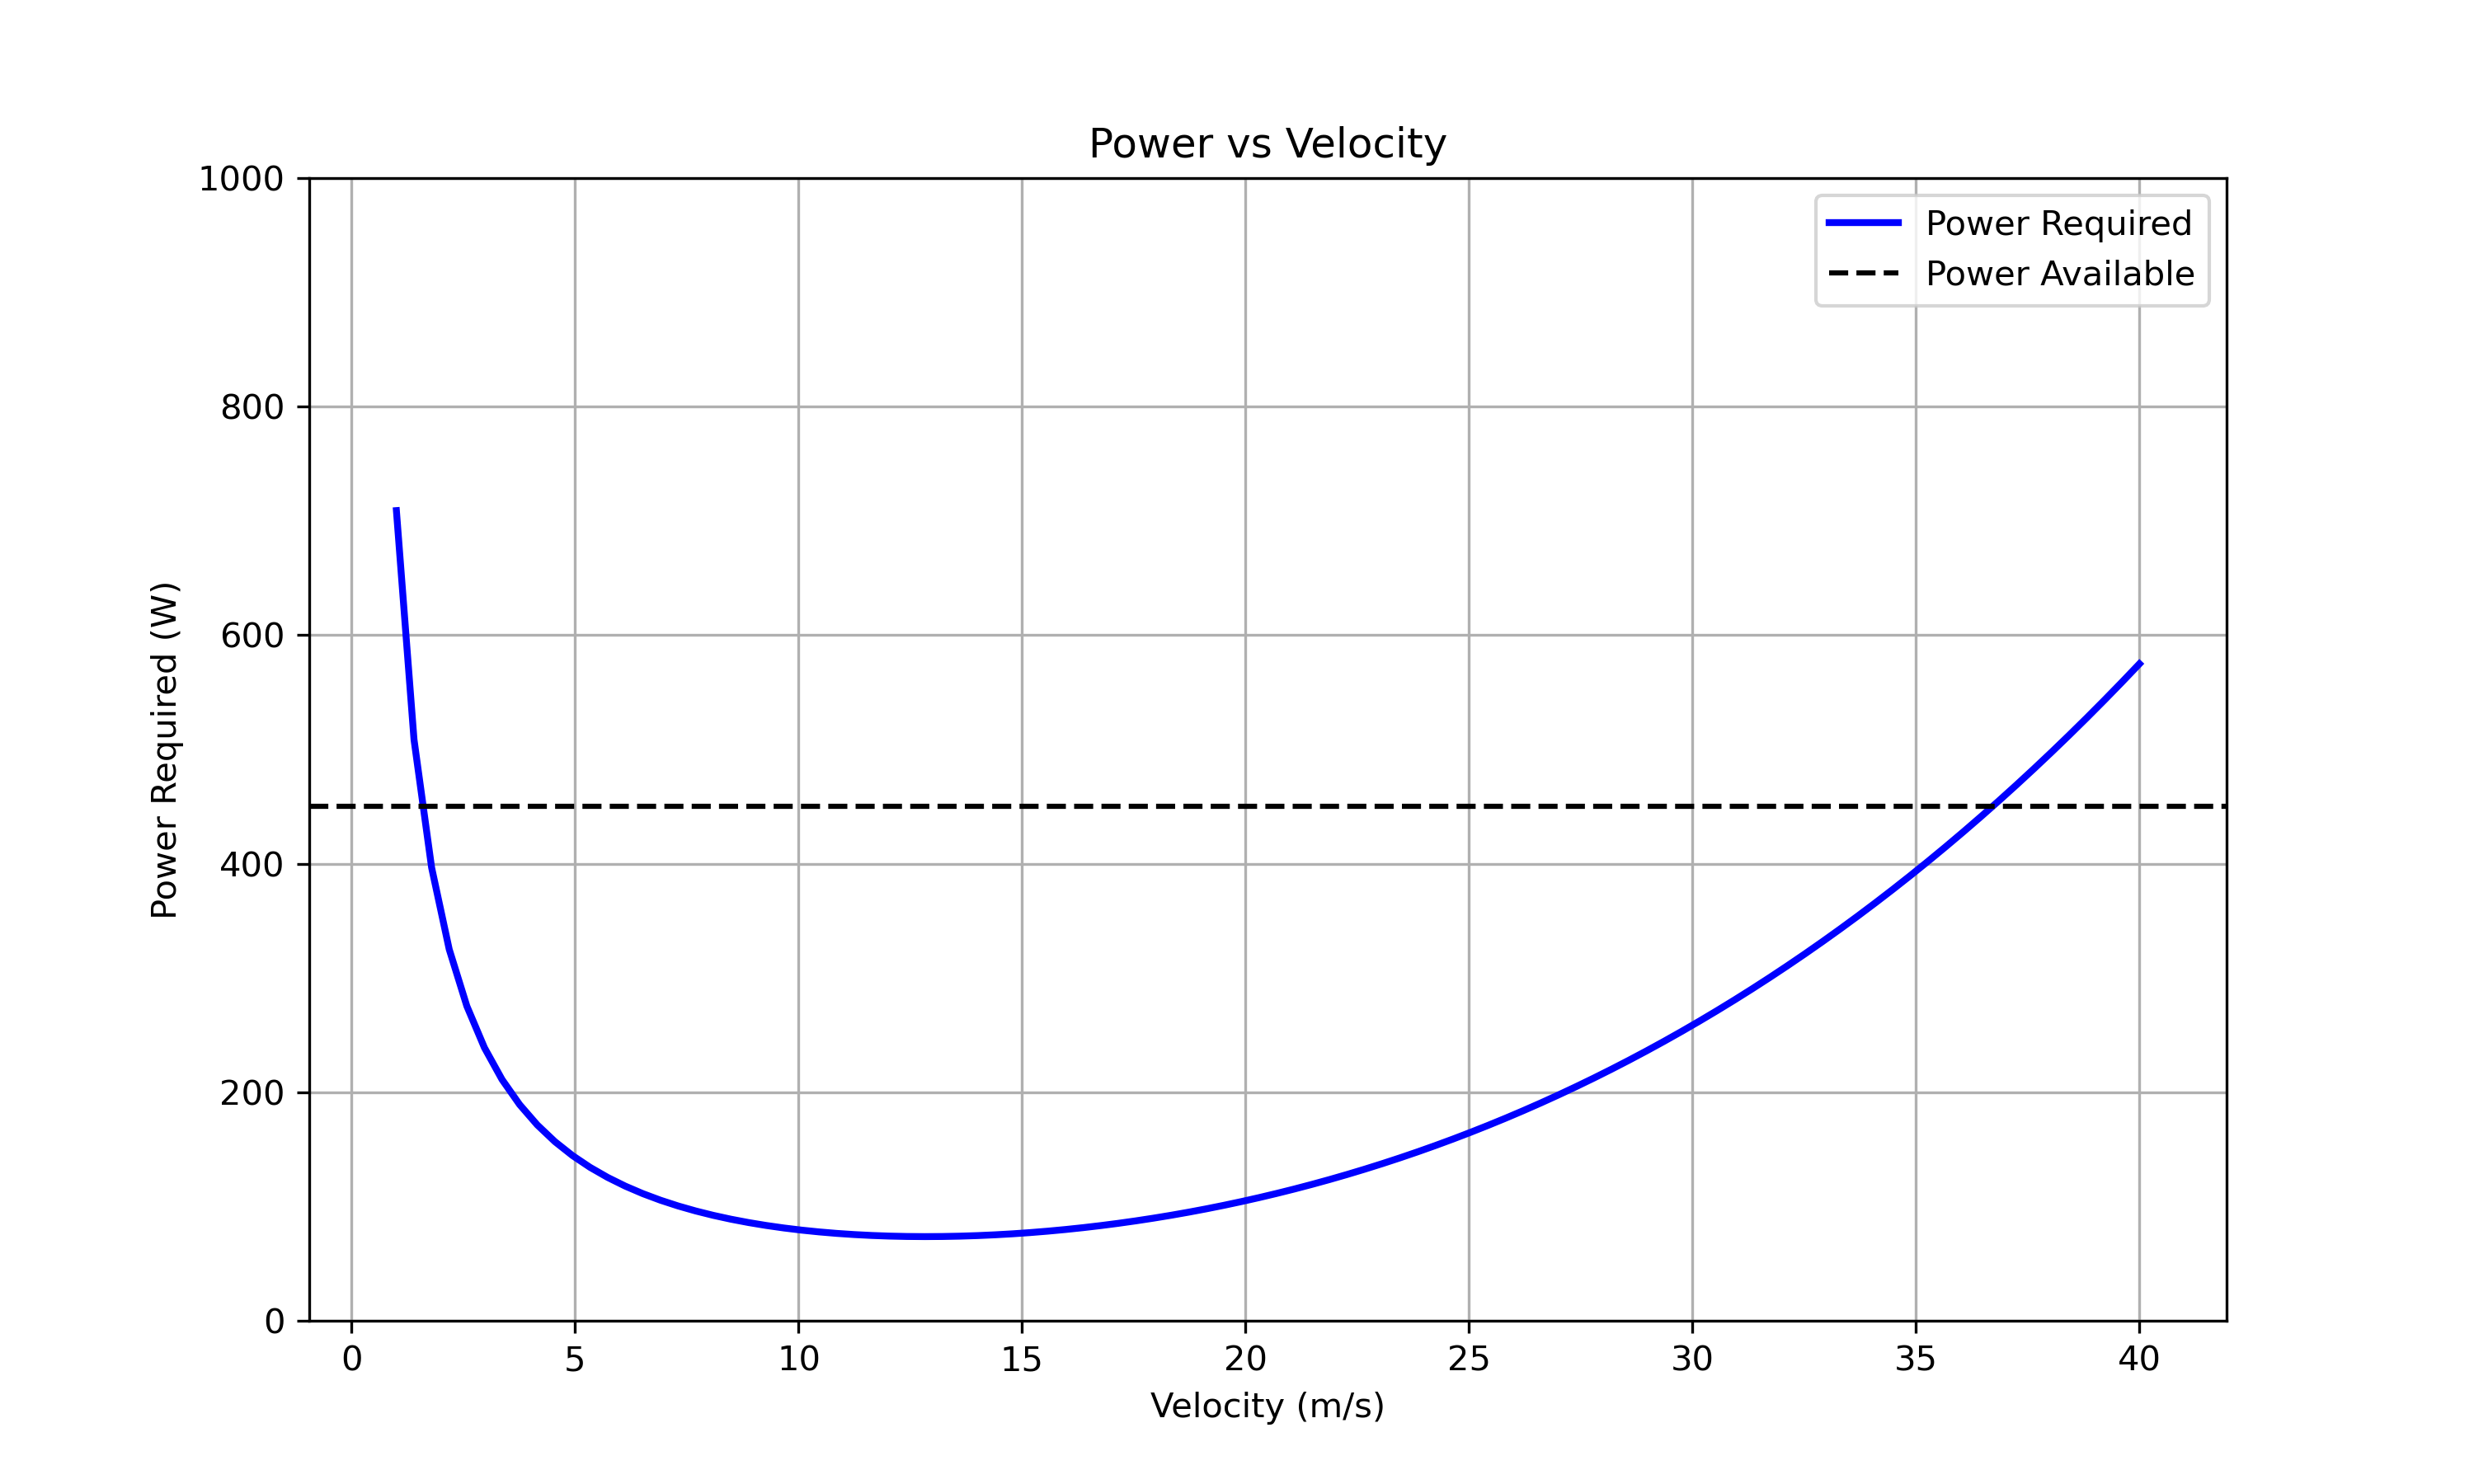
\includegraphics[width=\linewidth,height=0.45\textheight,keepaspectratio]{Power_vs_Velocity.png}
  \end{figure}
\end{columns}
\end{frame}

\begin{frame}[t]{Performance II: Rate of Climb}
\begin{columns}[T,onlytextwidth]
  \column{0.36\textwidth}
  \begin{block}{Climb performance}
  \small
  \begin{itemize}
    \item Rate of climb: \SI{3.5}{\meter\per\second}
    \item Optimal climb speed: \SI{16}{\meter\per\second}
    \item Climb angle: \SIrange{15}{20}{\degree}
    \item Takeoff distance: $<\SI{150}{\meter}$
  \end{itemize}
  \end{block}

  \begin{alertblock}{Takeaway}
  \small
  Climb performance is adequate for the mission and remains inside the available power margin.
  \end{alertblock}

  \column{0.62\textwidth}
  \begin{figure}
    \centering
    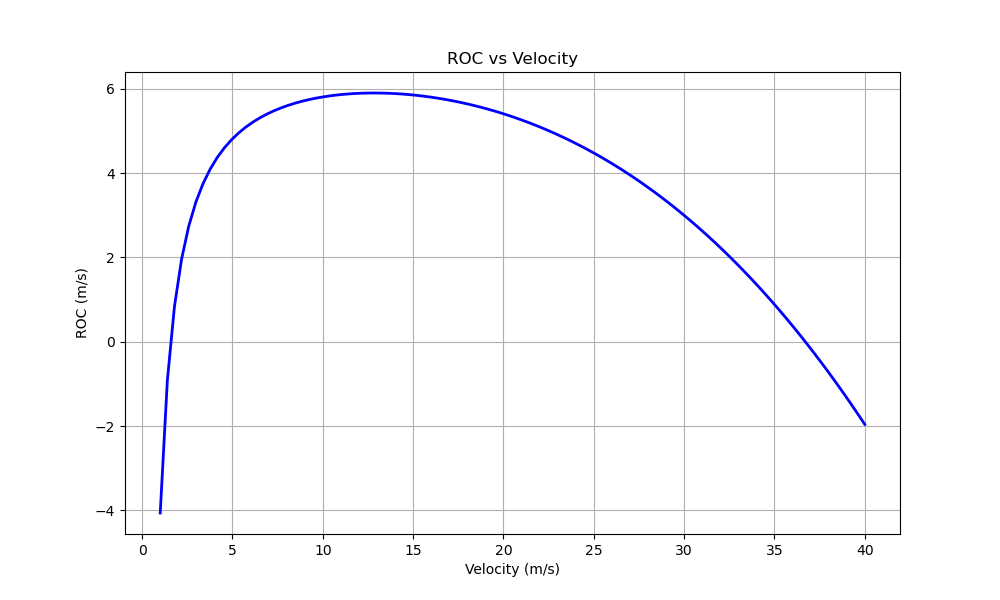
\includegraphics[width=\linewidth,height=0.42\textheight,keepaspectratio]{ROC_vs_Velocity.png}
  \end{figure}
\end{columns}
\end{frame}

% -------------------------------------------------
\begin{frame}[t]{Performance III: Load Factor and Takeoff Envelope}
\begin{columns}[T,onlytextwidth]
  \column{0.55\textwidth}
  \begin{figure}
    \centering
    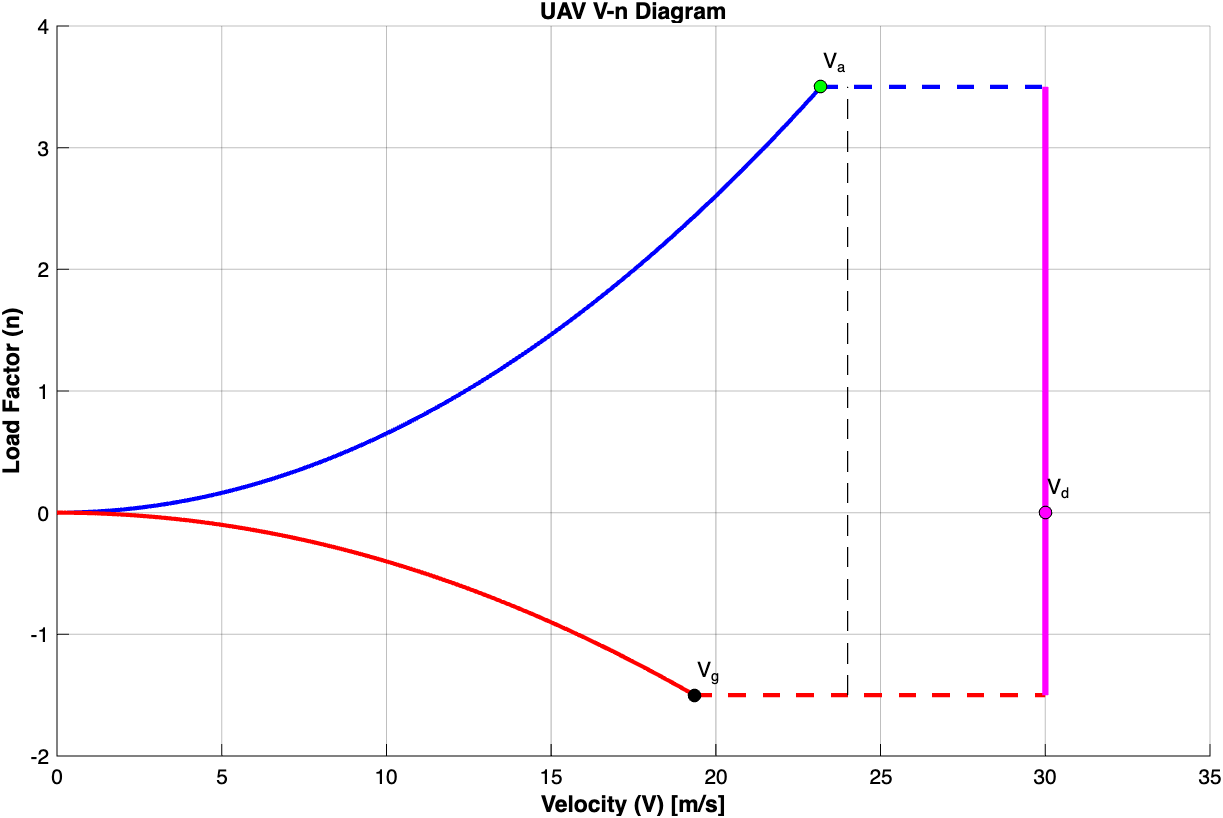
\includegraphics[width=\linewidth,height=0.55\textheight,keepaspectratio]{V_n_before_payload.png}
  \end{figure}
  \vspace{-0.5em}
  {\footnotesize\centering Positive maneuver envelope before payload release.\par}

  \column{0.41\textwidth}
  \begin{block}{Takeoff and landing}
  \small
  \begin{tabular}{@{}>{\bfseries}p{0.58\linewidth}p{0.26\linewidth}@{}}
    \toprule
    Takeoff distance & $<\SI{150}{\meter}$ \\
    Liftoff speed & \SI{13.6}{\meter\per\second} \\
    Landing distance & $<\SI{120}{\meter}$ \\
    Approach speed & \SI{15}{\meter\per\second} \\
    Positive limit load & 3.5 \\
    Negative limit load & -1.5 \\
    \bottomrule
  \end{tabular}
  \end{block}

  \begin{alertblock}{Operational takeaway}
  The aircraft satisfies the STOL requirement while retaining a practical speed margin for climb, cruise, and landing.
  \end{alertblock}
\end{columns}
\end{frame}

% -------------------------------------------------
\begin{frame}[t]{Stability I: Static Derivatives}
\begin{columns}[T,onlytextwidth]
  \column{0.48\textwidth}
  \begin{block}{Longitudinal stability}
  \small
  \begin{tabular}{@{}>{\bfseries}p{0.42\linewidth}p{0.46\linewidth}@{}}
    \toprule
    $C_{m_\alpha}$ & $-0.487~\mathrm{rad^{-1}}$ \\
    $C_{m_0}$ & 0.0125 \\
    $C_{m_q}$ & $-14.94~\mathrm{rad^{-1}}$ \\
    $C_{L_q}$ & $+5.66~\mathrm{rad^{-1}}$ \\
    $C_{D_\alpha}$ & $+0.104~\mathrm{rad^{-1}}$ \\
    \bottomrule
  \end{tabular}
  \end{block}

  \begin{exampleblock}{Interpretation}
  \small
  Negative $C_{m_\alpha}$ indicates static longitudinal stability, and the CG remains ahead of the neutral point.
  \end{exampleblock}

  \column{0.48\textwidth}
  \begin{block}{Lateral-directional stability}
  \small
  \begin{tabular}{@{}>{\bfseries}p{0.42\linewidth}p{0.46\linewidth}@{}}
    \toprule
    $C_{n_\beta}$ & $+0.0838~\mathrm{rad^{-1}}$ \\
    $C_{l_\beta}$ & $-0.0111~\mathrm{rad^{-1}}$ \\
    $C_{l_p}$ & $-0.659~\mathrm{rad^{-1}}$ \\
    $C_{n_r}$ & negative, stabilizing \\
    Roll damping & strong \\
    \bottomrule
  \end{tabular}
  \end{block}

  \begin{alertblock}{Interpretation}
  \small
  The sign pattern is consistent with weathercock stability, roll damping, and a conventional tail layout.
  \end{alertblock}
\end{columns}
\end{frame}

% -------------------------------------------------
\begin{frame}[t]{Stability II: Eigenvalue Analysis}
\begin{columns}[T,onlytextwidth]
  \column{0.48\textwidth}
  \begin{figure}
    \centering
    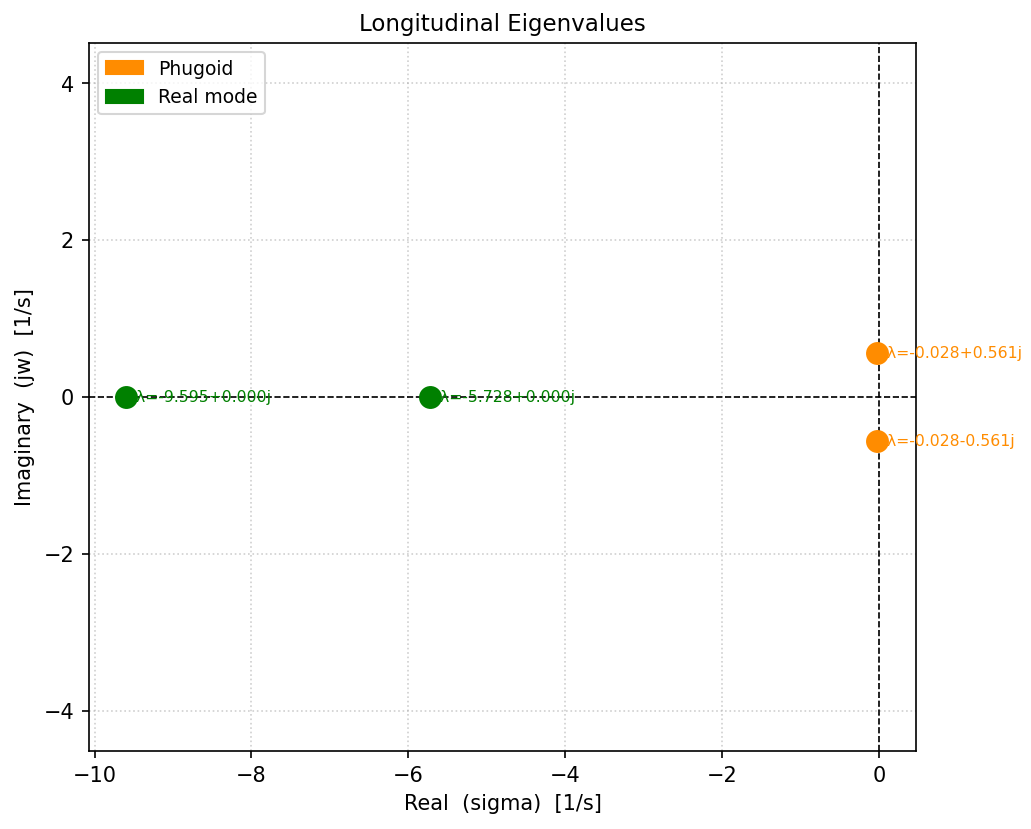
\includegraphics[width=\linewidth,height=0.39\textheight,keepaspectratio]{Longitudinal_eigenvales.png}
  \end{figure}
  \vspace{-0.6em}
  {\footnotesize\centering Longitudinal modes: phugoid and real mode.\par}

  \column{0.48\textwidth}
  \begin{figure}
    \centering
    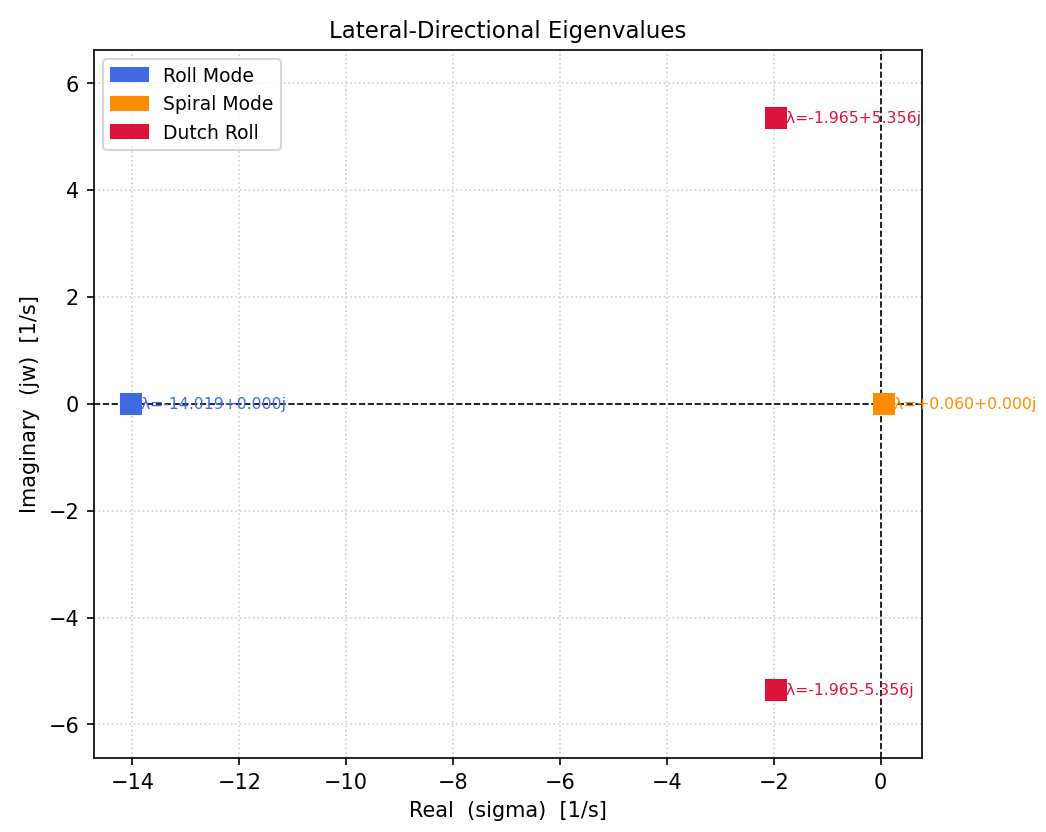
\includegraphics[width=\linewidth,height=0.39\textheight,keepaspectratio]{Lateral_eigenvalues.png}
  \end{figure}
  \vspace{-0.6em}
  {\footnotesize\centering Lateral-directional modes: roll, spiral, and Dutch roll.\par}
\end{columns}

\begin{center}
\scriptsize
\begin{tabular}{@{}lll@{}}
\toprule
\textbf{Mode} & \textbf{Key result} & \textbf{Interpretation} \\
\midrule
Phugoid & lightly damped & expected for small UAV \\
Roll mode & fast decay & strong roll stabilization \\
Dutch roll & stable complex pair & acceptable damping \\
Spiral mode & slightly unstable / slow & monitor in trim and control tuning \\
\bottomrule
\end{tabular}
\end{center}
\end{frame}

% -------------------------------------------------
\begin{frame}[t]{Isometric CAD Views}
\begin{columns}[T,onlytextwidth]
  \column{0.50\textwidth}
  \begin{figure}
    \centering
    \cadplaceholder{Isometric view placeholder}
  \end{figure}
  \begin{figure}
    \centering
    \cadplaceholder{Top view placeholder}
  \end{figure}

  \column{0.50\textwidth}
  \begin{figure}
    \centering
    \cadplaceholder{Side view placeholder}
  \end{figure}
  \begin{figure}
    \centering
    \cadplaceholder{Front view placeholder}
  \end{figure}
\end{columns}

\begin{block}{Integration notes}
\small
The final CAD package should show the payload bay, propulsion placement, landing gear clearance, control surfaces, and avionics access.
\end{block}
\end{frame}

% -------------------------------------------------
\begin{frame}[t]{Requirements Compliance Summary}
\small
\renewcommand{\arraystretch}{1.12}
\begin{tabularx}{\textwidth}{@{}>{\bfseries}X >{\centering\arraybackslash}p{2.3cm} >{\centering\arraybackslash}p{2.7cm} >{\centering\arraybackslash}p{0.9cm}@{}}
\toprule
Requirement & Target & Achieved & Status \\
\midrule
Maximum wingspan & \SI{2.00}{\meter} & \SI{2.00}{\meter} & \ok \\
Payload capacity & \SIrange{1}{2}{\kilo\gram} & \SI{1.20}{\kilo\gram} & \ok \\
Operational radius & \SIrange{40}{50}{\kilo\meter} & \SI{41.6}{\kilo\meter} & \ok \\
Total range & \SIrange{80}{100}{\kilo\meter} & \SI{83.15}{\kilo\meter} & \ok \\
Endurance & \SIrange{1}{2}{\hour} & 2 h 5 min & \ok \\
Cruise speed & \SIrange{18}{25}{\meter\per\second} & \SIrange{18}{22}{\meter\per\second} & \ok \\
Takeoff distance & $<\SI{150}{\meter}$ & $<\SI{150}{\meter}$ & \ok \\
Static stability & positive margin & \(\approx 14\%\) MAC & \ok \\
\bottomrule
\end{tabularx}

\vspace{0.3em}
\begin{center}
\begin{beamercolorbox}[rounded=true,shadow=true,wd=0.84\textwidth,center,sep=0.55em]{block body}
\small\parbox{0.76\textwidth}{\centering\textcolor{navymain}{\textbf{Overall conclusion:}} the conceptual UAV meets the mission, range, payload, STOL, and stability goals.}
\end{beamercolorbox}
\end{center}
\end{frame}

% -------------------------------------------------
\begin{frame}[plain]
\vfill
\begin{center}
{\fontsize{20}{24}\selectfont\bfseries Thank you}\\[0.2cm]
{\large Questions?}
\end{center}
\vfill
\end{frame}

\end{document}
